\section{Cipher Specifications}

\begin{frame}[c]{Cipher Design}
\begin{itemize}
    \item PRESENT-80 is an example of SP-network.
    \item 4-bit S-Box is applied 16 times in parallel for the 64-bit input during each round.
    \begin{block}{High level psuedo-code of PRESENT algorithm}
        \begin{algorithmic}[1]
        \STATE{generateRoundKeys()}
        \FOR{$i=1$ \TO $31$ }
            \STATE {addRoundKey(\textsc{State},$K_i$)}
            \STATE {sBoxLayer(\textsc{State})}
            \STATE {pLayer(\textsc{State})}
        \ENDFOR
        \STATE addRoundKey(\textsc{State},$K_{32}$)
        \end{algorithmic}
    \end{block}
\end{itemize}
\end{frame}

\begin{frame}{Cipher Design contd.}
       \begin{block}{Add Round Key}
           \begin{itemize}
               \item Round key $K_i = k_{63},k_{62} \dots k_0$ for $1\leq i \leq 32$.
               \item Current state $S = s_{63},s_{62}\dots s_0$.
               \begin{eqnarray*}
                    S \xrightarrow{} S \oplus K_i \\
                    \implies s_t \xrightarrow[]{} s_t \oplus k_t
                \end{eqnarray*}
                for $0\leq t\leq 63$
           \end{itemize}
       \end{block}
\end{frame}

\begin{frame}{Substitution Layer}
     PRESENT S-Box satisfies the following conditions.
    \begin{itemize}
        \item For any fixed input difference $\Delta_I \in \mathbb{F}_2^4,\Delta_I \not = 0$ and output difference $\Delta_O \in \mathbb{F}_2^4,\Delta_I \not = 0$, the following condition is satisfied
        \begin{equation*}
            |\{ x \in \mathbb{F}_2^4~~ \vert~~ S(\Delta_I +x) + S(x) = \Delta_O \}| \leq 4
        \end{equation*}
        \item For any fixed input difference $\Delta_I \in \mathbb{F}_2^4,\Delta_I \not = 0$ and output difference $\Delta_O \in \mathbb{F}_2^4$ such that $wt(\Delta_O) = wt(\Delta_I) = 1$, the following condition is satisfied
        \begin{equation*}
            \{ x \in \mathbb{F}_2^4~~ \vert~~  S(\Delta_I +x) + S(x) = \Delta_O  \} = \Phi
        \end{equation*}
        where $wt(x)$ is the hamming weight of $x$.
    \end{itemize}
\end{frame}

\begin{frame}{Cipher Design Contd.}
    \begin{block}{Permutation Layer}
        \begin{itemize}
            \item Bit permutation.
            \item Bit $i$ of \textsc{STATE} is moved to bit position $P(i)$.
        \end{itemize}
        \begin{eqnarray*}
         P(i) =  \begin{cases}
              16.i~~ mod~~ 63 & i \in \{0,1,\dots 62 \}\\
              63 & i = 63
           \end{cases}
        \end{eqnarray*}
    \end{block}
\end{frame}


\begin{frame}{Key schedule Algorithm}
We discuss the 80-bit key schedule algorithm.
 \begin{figure}[H]
	\centering
	\minipage{\textwidth}
	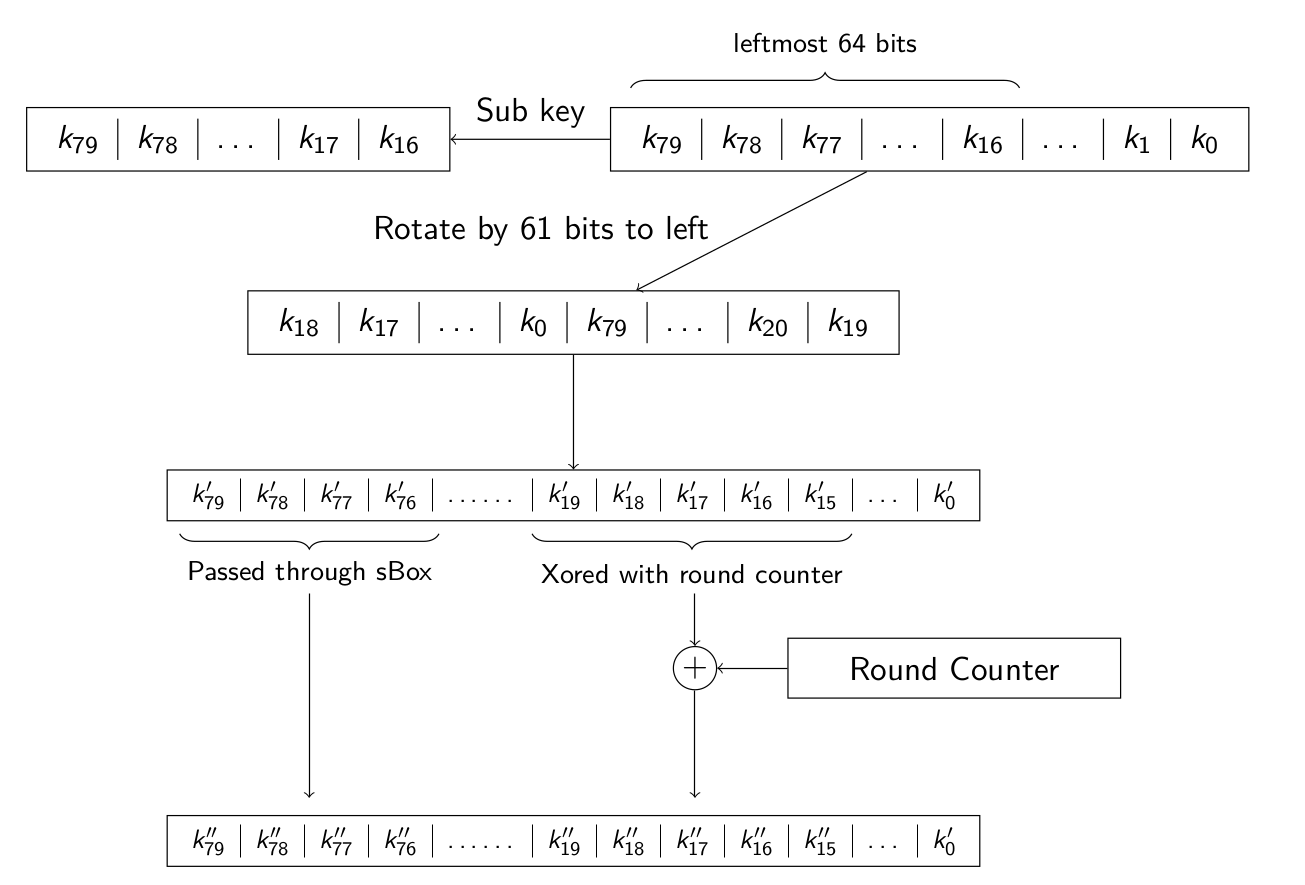
\includegraphics[width=\linewidth]{key.png}
	\endminipage
	\caption{Key schedule}
	\label{fig:key}
\end{figure}
\end{frame}
